\documentclass[border=6pt]{standalone}
\usepackage{tikz}
\usetikzlibrary{arrows.meta,calc}
% Okabe-Ito palette, readable by colour blind viewers
\definecolor{cg}{HTML}{E69F00}
\definecolor{cn}{HTML}{009E73}
\definecolor{cf}{HTML}{0072B2}
\definecolor{ca}{HTML}{D55E00}
\definecolor{cacc}{HTML}{CC79A7}
\begin{document}
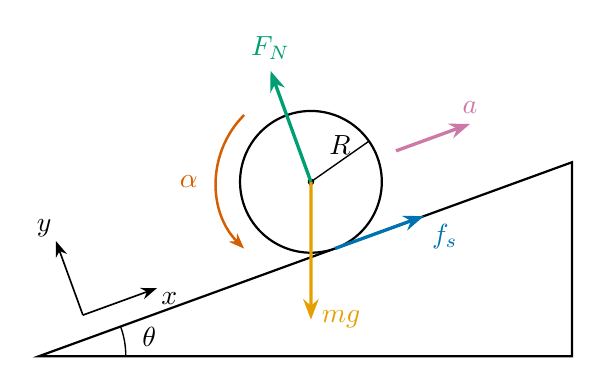
\begin{tikzpicture}[
  force/.style={-{Stealth[length=2.6mm]}, line width=1.2pt},
  axis/.style={-{Stealth[length=2mm]}, line width=0.6pt},
  thin/.style={line width=0.5pt}
]
\def\th{20}
\def\L{7.2}
\def\R{0.9}
\def\s{4.0}
% incline
\draw[line width=0.8pt] (0,0) -- ({\L*cos(\th)},0) -- ({\L*cos(\th)},{\L*sin(\th)}) -- cycle;
\draw[thin] (1.1,0) arc (0:\th:1.1);
\node at ({1.42*cos(\th/2)},{1.42*sin(\th/2)}) {$\theta$};

\begin{scope}[rotate=\th]
  \coordinate (c) at (\s,\R);
  \coordinate (p) at (\s,0);
  % axes
  \draw[axis] (0.7,0.3) -- ++(1.0,0) node[below right=-2pt] {$x$};
  \draw[axis] (0.7,0.3) -- ++(0,1.0) node[above left=-2pt] {$y$};
  % ball
  \draw[line width=0.8pt, fill=white] (c) circle (\R);
  \fill (c) circle (1.2pt);
  \draw[thin] (c) -- ($(c)+(15:\R)$) node[midway, above=-1pt] {$R$};
  % accelerations
  \draw[axis, ca, line width=0.9pt] ($(c)+(115:{\R+0.3})$) arc (115:205:{\R+0.3});
  \node[ca] at ($(c)+(160:{\R+0.65})$) {$\alpha$};
  \draw[force, cacc] ($(c)+({\R+0.25},0)$) -- ++(1.0,0) node[above] {$a$};
  % forces
  \draw[force, cg] (c) -- ($(c)+(250:1.75)$) node[right] {$m g$};
  \draw[force, cn] (c) -- ++(0,1.5) node[above] {$F_N$};
  \draw[force, cf] (p) -- ++(1.2,0) node[below right=-1pt] {$f_s$};
\end{scope}
\end{tikzpicture}
\end{document}
